\documentclass{astroedu-lab}

\begin{document}

\pagestyle{plain}

\begin{problem}{\huge Лабораторная работа 4.2.3\\\\Интерферометр Релея\\\\Выполнил Жданов Елисей Б01-205}

\section{Цель работы:}

Ознакомление с интерференцией на двух щелях,
устройством и принципом действия интерферометра Релея и с его
применением для измерения показателей преломления газов.


\section{Оборудование:}

Технический интерферометр ИТР-1, светофильтр, баллон с углекислым газом, сильфон, манометр, краны.

\section{Теоретическая справка}

Зависимость показателя преломления газа от давления и температуры. Воспользуемся известной формулой диэлектрической проницаемости $\varepsilon$ для газа невзаимодействующих диполей:
$$
\varepsilon=n^2=1+4 \pi N \alpha,
$$

где $N$ - концентрация молекул, $\alpha$ - поляризуемость молекулы (в ед. СГС). Эта формула справедлива для разреженных газов, и коэффициент преломления их мало отличается от единицы. Учитывая зависимость давления $P$ газа от температуры $P=N k_{\mathrm{B}} T$, где $k_{\mathrm{b}}$ - константа Больцмана, получим соотношение
$$
n-1 \approx \frac{\alpha}{2 k_{\mathrm{B}} T} P .
$$

Тогда для разности показателей преломления $\delta n=n_2-n_1$, измеряемой с помощью интерферометра Релея, и разности давлений $\delta P$, измеряемой с помощью манометра, имеем простое соотношение:
$$
\delta n=\frac{\alpha}{2 k_{\mathrm{B}} T} \delta P .
$$

\section{Экспериментальная установка}

\begin{figure}[!h]
	\centering
	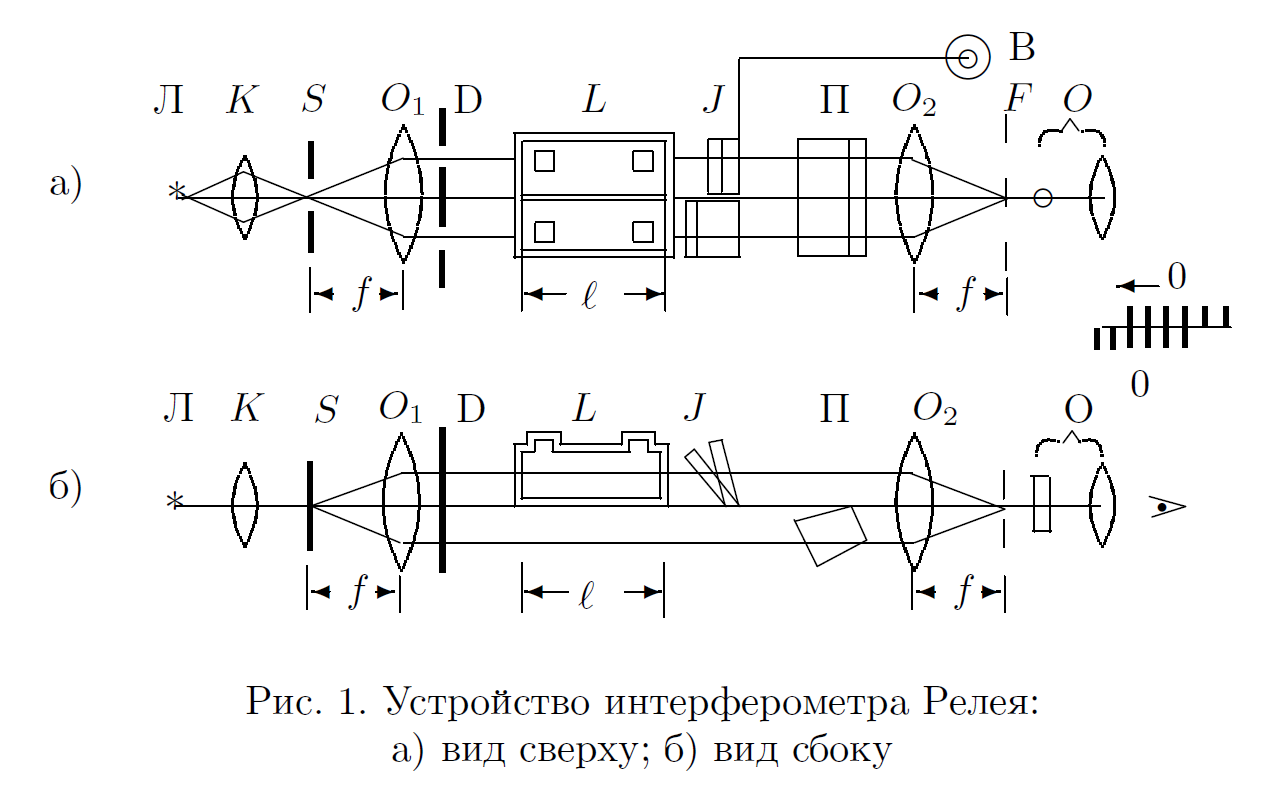
\includegraphics[width=0.9\textwidth]{установка.png}
	\label{fig:boiler}
\end{figure}

Интерферометр Релея - прибор для измерения разности показателей преломления - основан на явлении дифракции света на двух параллельных щелях. Схема прибора представлена на рис. 1 в вертикальной и горизонтальной проекциях. Лампа накаливания Л с помощью конденсора $K$ ярко освещает узкую входную щель $S$, расположенную в фокусе объектива $O_1$ (фокусное расстояние $f$ ). Коллиматор, состоящий из щели $S$ и объектива $O_1$, посылает параллельный пучок на диафрагму $D$ с двумя вертикальными щелями (расстояние между щелями $d$ ). Свет после двойной щели проходит кювету $L$, состоящую из двух одинаковых стеклянных камер, в которые вводятся исследуемые газы (в нашей установке - $\mathrm{CO}_2$ или воздух). Кювета занимает только верхнюю часть пространства между объективами $\mathrm{O}_1$ и $\mathrm{O}_2$, длина кюветы $\ell$. За кюветой расположены две стеклянные пластинки $J$ (компенсатор Жамена, см. ниже) и пластинка П.

Интерференционная картина (картина дифракции на двух щелях), наблюдаемая в фокальной плоскости $F$ объектива $O_2$, представляет собой две системы равноотстоящих полос, параллельных щелям: верхняя (подвижная) образована лучами, прошедшими через кювету, нижняя (неподвижная) - лучами, прошедшими под кюветой. Обе системы интерференционных полос разграничены при помощи пластины П тонкой разделительной линией. Для наблюдения двух систем полос в окуляре применена цилиндрическая линза диаметром 2,2 мм, ось которой расположена вертикально. Вторая («глазная») линза окуляра - обычная сферическая. Она служит для подстройки чёткости картины под глаз наблюдателя.

При малых дифракционных углах $\varphi=\lambda / d$ расстояние между соседними светлыми (или тёмными) полосами $\delta y$ зависит от длины волны $\lambda$, фокусного расстояния $f$ объектива $O_2$ и расстояния между дифракционными щелями $d$ :
$$
\delta y=f \frac{\lambda}{d} .
$$

В техническом интерферометре ИТР-1, который используется в нашей работе, $f \simeq 20 \mathrm{~cm}, d \simeq 1,5 \mathrm{~cm}$, и $\delta y$ оказывается порядка $10^{-3}$ см. Для наблюдения таких мелких интерференционных полос требуется окуляр с большим увеличением ( $\gamma \simeq 150^{\times}$). Короткофокусная цилиндрическая линза окуляра О сильно растягивает интерференционную картину по горизонтали, не меняя её вертикальных размеров и тем самым мало ослабляя освещённость полос. Изображение светящейся точки в фокальной плоскости объектива $O_2$ при рассматривании через цилиндрическую линзу имеет вид светлой вертикальной линии, длина которой определяется диаметром объектива. Поэтому распределение освещённости в нижней части светлой линии зависит от действия нижней части объектива, а в верхней части линии - от верхней части объектива. Таким образом, наблюдатель видит две системы полос: верхняя образована лучами, прошедшими через кюветы, нижняя - лучами, прошедшими под кюветами.

При заполнении камер газами с одинаковым показателем преломления $n$ обе системы полос совпадают. Оптическая разность хода $\Delta=\delta n \cdot l$, возникающая при прохождении света через камеры с разными газами $\delta n=n_2-n_1$, ведёт к поперечному смещению верхней дифракционной картины относительно неподвижной нижней. Смещение на одну полосу соответствует дополнительной разности хода $\Delta=\lambda$. Просчитав число полос $m$ между центрами обеих картин, можно рассчитать
$$
\delta n=\frac{\Delta}{\ell}=m \frac{\lambda}{\ell} .
$$

Для точного измерения разности хода используется компенсатор Жамена ( $J$ на рис. 1) - устройство, которое позволяет вернуть подвижную систему полос к первоначальному положению, т. е. вновь совместить обе системы полос. В установке компенсатор Жамена расположен за кюветой. Он состоит из двух одинаковых плоскопараллельных стеклянных пластинок, установленных на пути лучей под углом $45^{\circ}$ к горизонтали. Вращение одной из пластин вокруг горизонтальной оси, перпендикулярной оси системы, вызывает увеличение или уменьшение оптической длины пути соответствующего луча. Ось вращения снабжена рычагом, конец которого смещается при помощи микрометрического винта В.

Интерферометр Релея можно применять для измерения небольших изменений показателей преломления жидкостей или газов, а также для определения примесей различных газов в воздухе (например, для измерения концентрации рудничного газа в шахте). Показатель преломления $n$ исследуемого газа определяется путём сравнения с воздухом при атмосферном давлении:
$$
n=n_{\text {возд }}+\frac{\Delta}{\ell} .
$$

Для определения величины $\Delta$ компенсатор следует прокалибровать.

\section{Измерения, Обработка}

1)

Построим калибровочный график, отложив по оси абсцисс номер сов-
мещённой полосы m, а по оси ординат величину z (отсчёт по компен-
сатору)

\begin{figure}[!h]
	\centering
	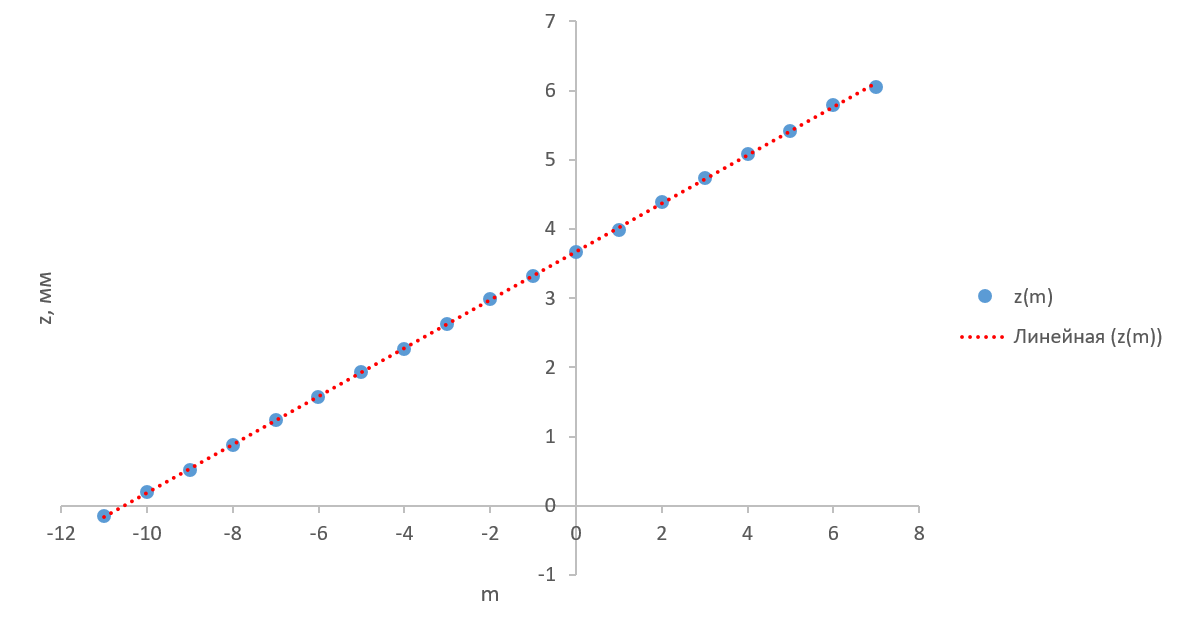
\includegraphics[width=1\textwidth]{mz.png}
	\label{fig:boiler}
\end{figure}

Линейность графика действительно сохраняется вдали от нулевого положения компенсатора(разброс точек случаен вдоль всей линеаризационной прямой)

Аппроксимация по МНК:

Найдем угловые коэффициенты прямых для каждой установки по МНК.

\[
	a = \frac{<x_i y_i> - < x > < y_i >}{< x_i^2> - < x_i >^2}
\]

\[
	b = < \nu_i > - a < N_i >
\]

Также рассчитаем их погрешности

\begin{equation}
	S_a^2 = \frac{< x_i^2>}{< x_i^2 > - < x_i >^2} \cdot \frac{<  b_i - b > ^2}{n - 2}
\end{equation}

\begin{equation}
	z = (3.6705 \pm 0.0053) + (0.34842 \pm 0.00091) \cdot m
\end{equation}

Коэффициент наклона будет использоваться для пересчета количества полос между двумя положениями микрометра.

2) Длина волны светового фильтра $\lambda = 656$ нм.

Длина кюветы l = 25 см

Рассчитаем зависимость $\delta n (\Delta P)$ и построим график

\begin{figure}[!h]
	\centering
	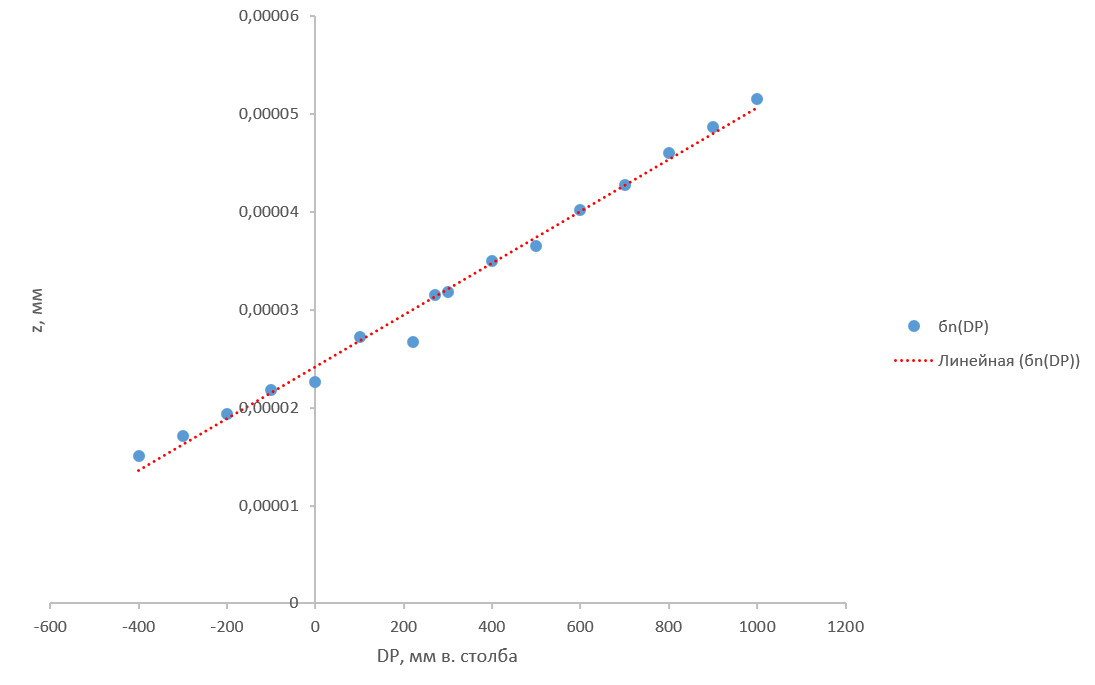
\includegraphics[width=1\textwidth]{dnDP.png}
	\label{fig:boiler}
\end{figure}

Аппроксимация по МНК (с учетом выбросов)

\begin{equation}
	\delta n = (0.00002445 ± 2.4e-7) + (2.639e-8 ± 4.6e-10)\cdot \Delta P
\end{equation}

По коэффициенту наклона рассчитаем поляризуемость "молекул воздуха".

\begin{equation}
	\frac{\delta n}{\Delta P} = \frac{\alpha}{2 k_b T}
\end{equation}

\begin{equation}
	\alpha = k \cdot 2 k_b T = (1.63 \pm 0.03) \cdot 10^{-30} \text{ м}^3
\end{equation}

Температура в лаборатории $T = 22.4 ^\circ$ С 

Давление в лаборатории $P_0 = 101900$ Па.

Посчитаем показатель преломления

\begin{equation}
	n = 1 + \frac{\alpha}{2 k_b T} P = (1.00027 \pm 0.00005)
\end{equation}

Что сходится с табличным значением

3) Приведу зависимость, связанную с концентрацией $CO_2$ от времени

\begin{figure}[!h]
	\centering
	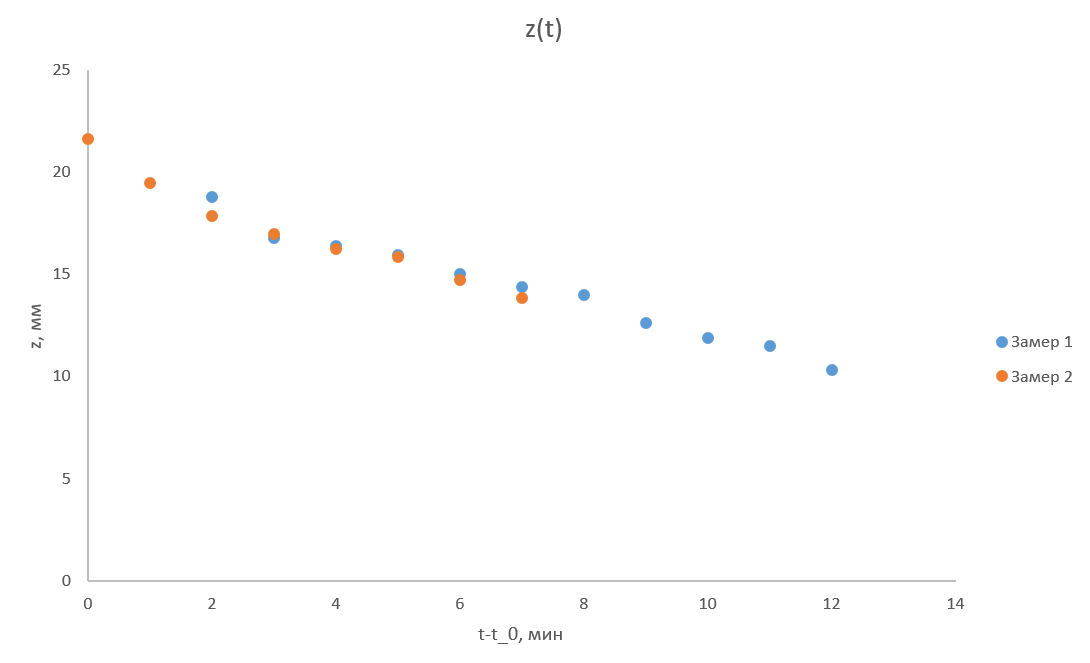
\includegraphics[width=1\textwidth]{co2.png}
	\label{fig:boiler}
\end{figure}

Взяв максимальное $z = 21.65$ мм, получим показатель преломления $CO_2$

\begin{equation}
	n = (1.0004 \pm 0.0001)
\end{equation}

Что также довольно близко к табличному значению 1.00045

\section{Вывод}

Интерферометр Релея действительно может с высокой точностью измерять показатели преломления, в частности, газов.

\section{Ресурсы}

Расчет по МНК: метод-наименьших-квадратов.рф


\end{problem}
\end{document}